%图表序号清零
\setcounter{table}{0}
\setcounter{figure}{0}

\subsection{\hei\xiaosan\textbf{前期实验}}

  不同于其他一些传统的黑盒机器学习方法,卷积网络所提取的
  图像特征在训练过程中是可视的,这不仅让人们对于卷积网络的工作过程
  有直观的了解,更能够帮助进行下一步的工作。
  % 在卷积网络的前向传播过程中部分卷积层滤波器提取的特征结果如图所示。
  % 这一部分本该插入训练过程中特征图的,但是特征图怎么都弄不出来,就作罢了
  % \begin{figure}[H]
  %   \centering
  %   \includegraphics[width=.45\textwidth, natwidth=674, natheight=404]{resource/second/data-ratio.bmp}
  %   \caption{数据分布}
  %   \label{Figure.Fourth.1}
  % \end{figure}

  为了改进本文模型的性能,在实验初期进行了不同迭代次数(分别为10000次、20000次)的实验,
  在图\ref{Figure.Fourth.1}(a)中以[橙-深蓝]、[红-浅蓝]图像对应其测试集和验证集的准确率;而
  [粉-绿]图像代表了卷积网络初步优化后的效果。验证准确率在70\%\textasciitilde75\%徘徊的
  原因来自于数据集:因为数据来自百度和谷歌图库,而这些图片是从各个网页上收集而来,其中大
  多数含有水印且画质模糊,为了收集到足够的实验用数据集,便在粗略挑选、裁剪后应用于实验,
  故此准确率不高。

  第一次训练对应的是[橙-深蓝]图象。该图像是在初步建立卷积网络模型的情况下训练的,
  由于输入数据较为粗糙,准确率只有65\%左右。由\ref{Figure.Fourth.1}(b)可以看出,
  在训练次数达到1500次时,验证损失率不降反升,这表明卷积网络模型存在过拟合的问题,
  而且在[红-浅蓝]图像中仍然存在该问题。[红-浅蓝]图像是训练了20000次的结果,在只有数据集
  稍微改进的情况下,验证准确率提升到72\%左右,但差别并不明显。

  在一些深度学习图像分类训练中,有的直接将测试集用作验证集,这可能有混淆概念的嫌疑。
  在调整数据集比例(训练集:测试集:验证集=3:1:1)后,又将输入图像的大小从
  $30\times30\times3$调整为$100\times100\times3$之后,便有了第三次的图像。
  从[粉-绿]图像可以明显看出,这次训练中用不到一千次迭代便将验证准确率提升至75\%,
  而测试准确率不到两千次便达到了99.84\%的准确率,远远好于前两次的训练效果。

    \begin{figure}[H]
      \centering
      \subfigure[训练-验证准确率]{
        \includegraphics[width=.45\textwidth]{resource/analysis/epoch_accuracy_small_1.eps}
      } %, natwidth=1259, natheight=822
      \subfigure[训练-验证损失率]{
        \includegraphics[width=.45\textwidth]{resource/analysis/epoch_loss_small_1.eps}
      } % , natwidth=1276, natheight=822
      \caption{卷积核的翻转对特征提取的影响}
      \label{Figure.Fourth.1}
    \end{figure}

  \subsection{\hei\xiaosan\textbf{参数优化}}
    在初步实验后,我们可以在图\ref{Figure.Fourth.1}中看到,现有模型的验证准确率仅
    在70\%左右徘徊,表现不尽人意。即使排除数据集的影响,也不能确说明该模型就是适合进行小麦病害
    图像分类的模型。
    % 况且对……。
    图\ref{Figure.Fourth.2}是在原卷积网络模型的基础上以不同学习率训练2000次绘出的。该图中橙、蓝、红
    分别对应学习率为$10^{-3}$、$5\times10^{-4}$、$10^{-4}$时的卷积网络模型。在模型表现方面,橙、蓝
    分别代表学习率为$10^{-3}$和$5\times10^{-4}$的模型解决了学习率为$10^{-4}$时出现的过拟合问题;
    在准确率方面,二者表现相差不大,但是在损失率的比对中,的比对中,但是在损失率的比对中,学习率
    $5\times10^{-4}$的模型表现更好。



    \begin{figure}[H]
      \centering
      \subfigure[验证准确率]{
        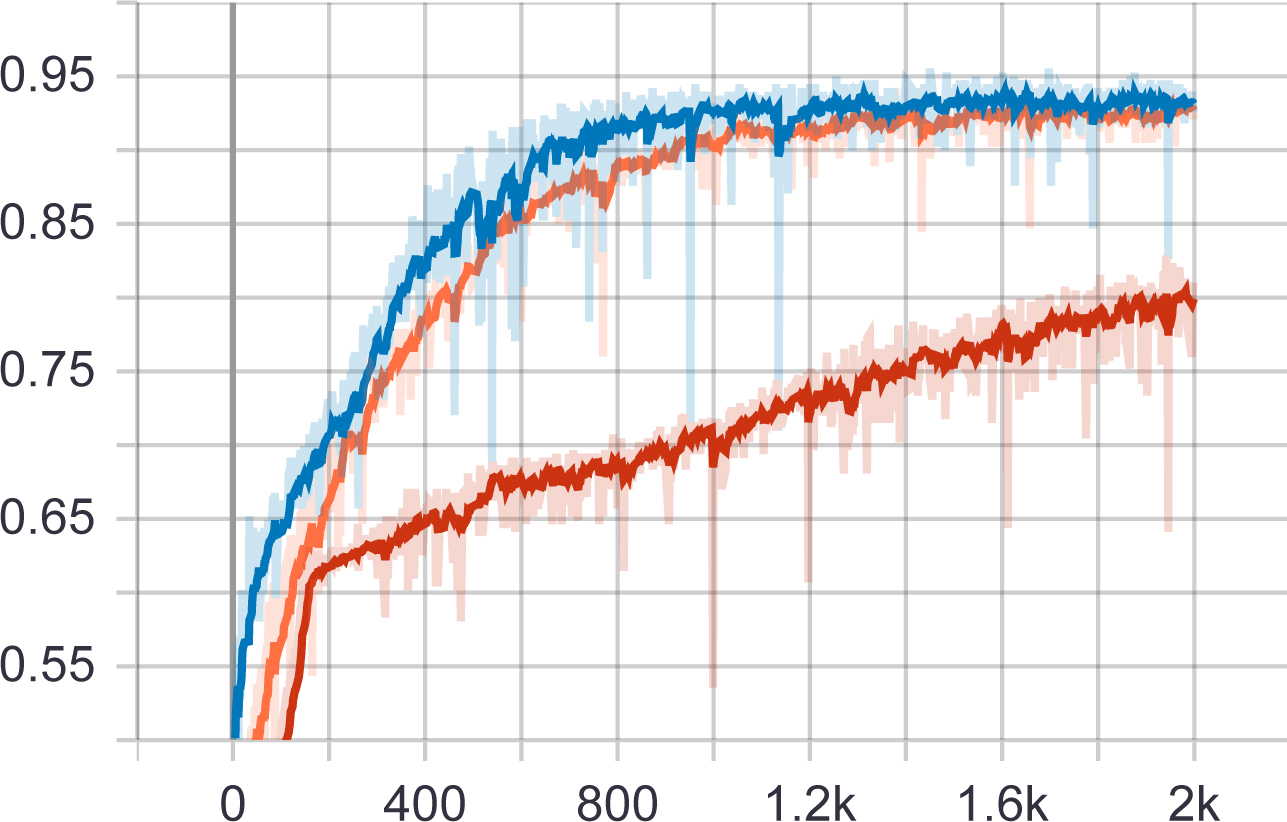
\includegraphics[width=.45\textwidth]{resource/analysis/epoch_val_acc_small.eps}
      }
      \subfigure[验证损失率]{
        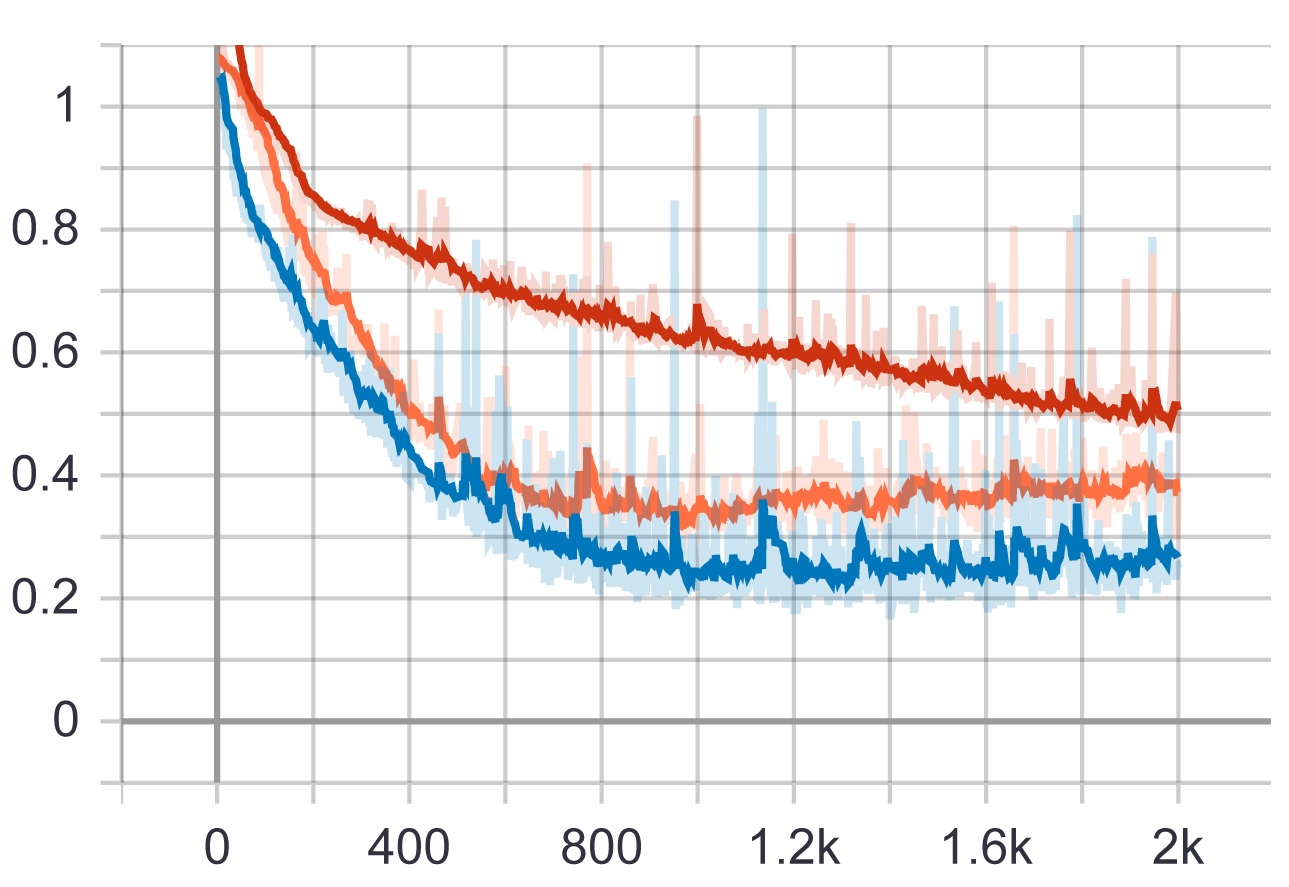
\includegraphics[width=.45\textwidth]{resource/analysis/epoch_val_loss_small.eps}
      }
      \caption{优化后准确率}
      \label{Figure.Fourth.2}
    \end{figure}

  \subsection{\hei\xiaosan\textbf{模型性能对比}}

    为了对比该模型在小麦病害图像分类的性能,在学习率$5\times10^{-4}$的背景下将其与合适的模型进行对比实验。
    图\ref{Figure.Fourth.3}中浅蓝代表LeNet-5、深蓝代表本文模型。LeNet-5运行次数较本文模型次数
    少的原因有二:第一,验证 准确率在400次之后就趋于平缓,不再有明显增长;第二,在200次之后验证
    损失率不降反升,具有过拟合的缺点,再继续训练已无意义。

    从分类模型的性能来看,LeNet-5的验证准确率约为84\%\textasciitilde85\%,本文模型约为93\%,稍高于
    LeNet-5;从另一方面来讲,现今的LeNet-5模型具有过拟合的缺点,200次训练后损失率不降反升。
    结合验证准确率和模型对比的结果,可以说本文提出的卷积网络模型更适合于处理小麦病害图像分类处理。

    \begin{figure}[H]
      \centering
      \subfigure[验证准确率]{
        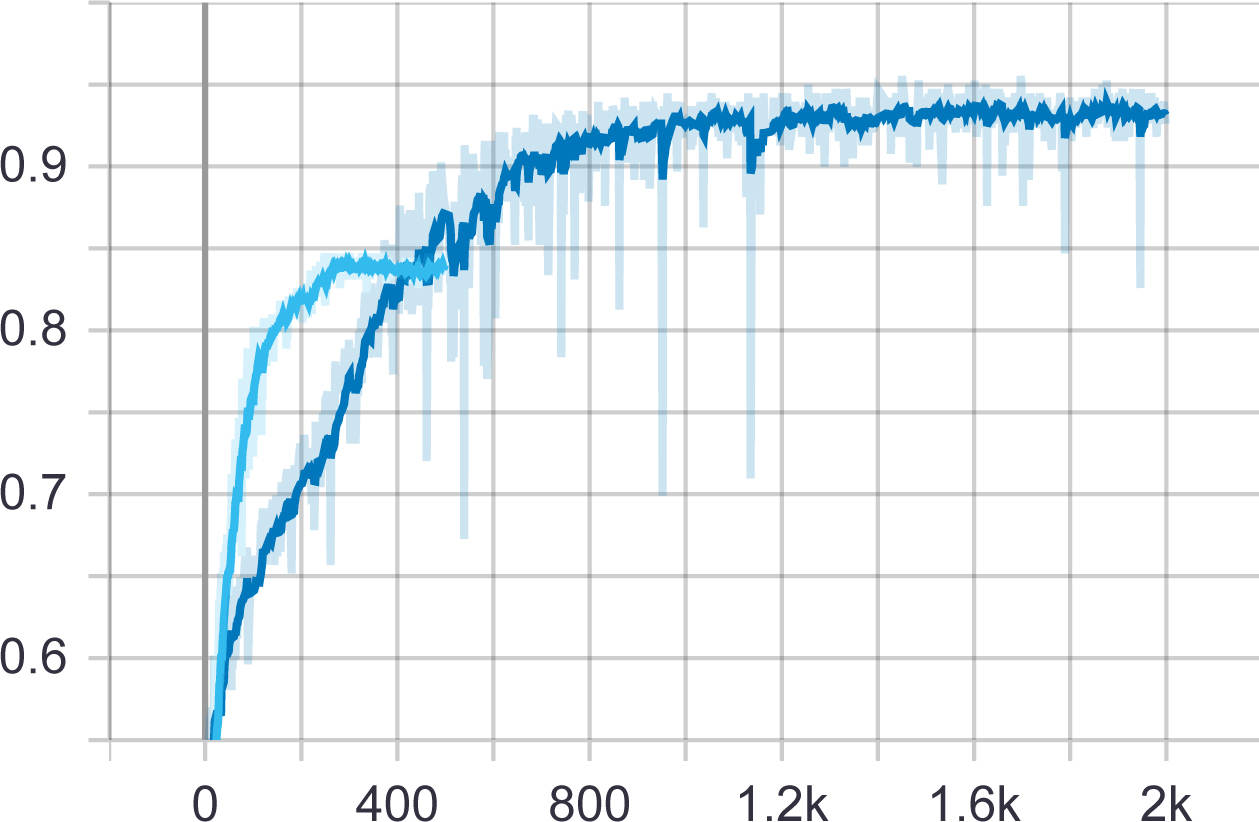
\includegraphics[width=.45\textwidth]{resource/analysis/lenet_newbnet_val_acc.eps}
      }
      \subfigure[验证损失率]{
        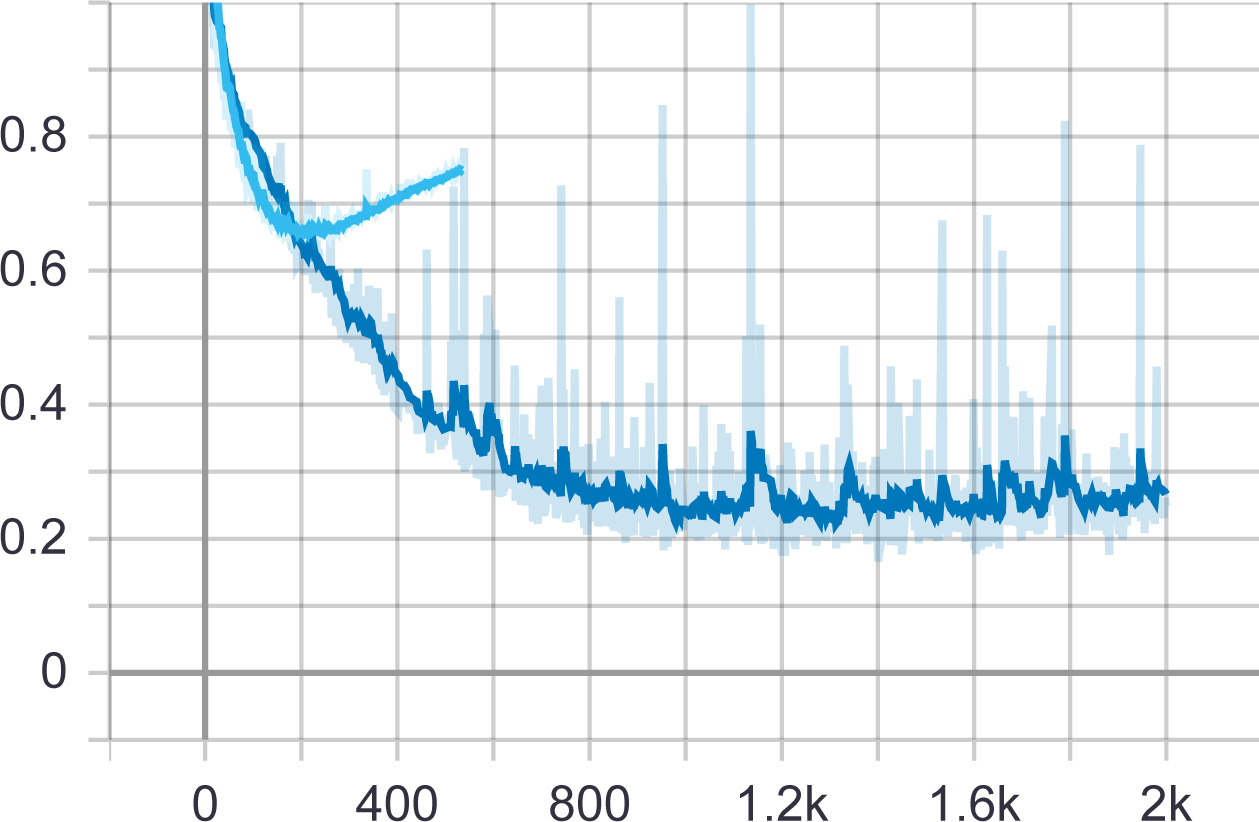
\includegraphics[width=.45\textwidth]{resource/analysis/lenet_newbnet_val_loss.eps}
      }
      \caption{LeNet-5与本文模型对比}
      \label{Figure.Fourth.3}
    \end{figure}


  \subsection{\hei\xiaosan\textbf{参数分布图}}
    图\ref{Figure.Fourth.4}展示了LeNet-5训练600次和本文模型训练2000次的卷积层偏置变化分布图。
    从图中可以看出,前者的偏置变化出现放缓的迹象,这说明该模型的权重已经收敛,模型也越来越确定
    当前的偏置为最适合本模型的值。而对本文模型的偏置变化来看,它仍然需要更多的训练次数来得到
    更精确的权重及偏置。
    这也说明了训练层次深的模型需要更多的训练次数,也需要更大的开销。
    从另一方面来讲,本模型在参数优化方面做的不够好,仍有待进行调整。

    \begin{figure}[H]
      \centering
      \subfigure[LeNet-5]{
        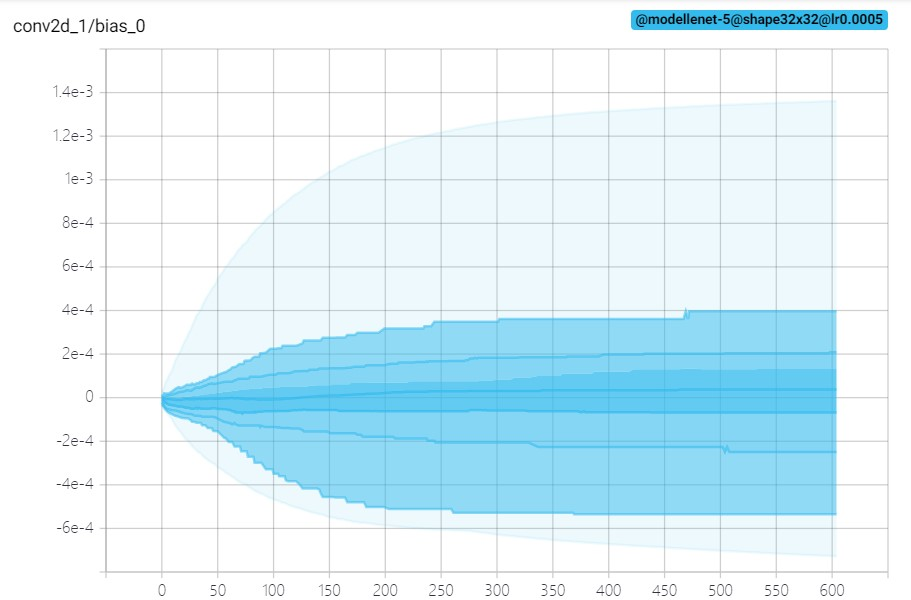
\includegraphics[width=.45\textwidth]{resource/analysis/distributions_lenet_conv2d_1_bias_0.jpg}
      }
      \subfigure[本文模型]{
        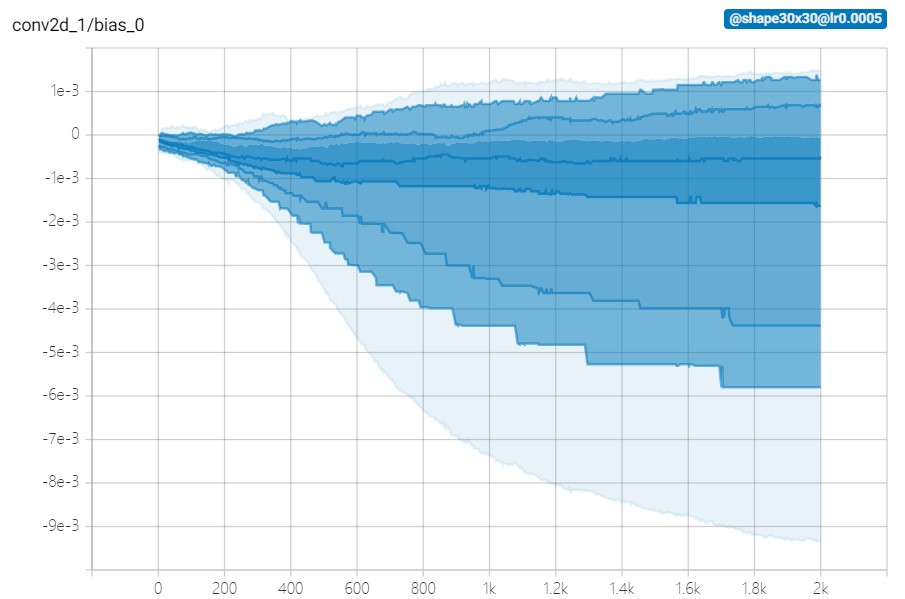
\includegraphics[width=.45\textwidth]{resource/analysis/distributions_newbnet_conv2d_1_bias_0.jpg}
      }
      \caption{2D分布图}
      \label{Figure.Fourth.4}
    \end{figure}
    
    直方图和分布图是同样的数据在不同维度的表现,从\ref{Figure.Fourth.5}可以看到,
    LeNet-5中的偏置自后向前逐渐减小,并在大约400次之后趋于平缓,不再有较大的变化,
    这意味着模型训练的完成。而就本文模型来看,偏置在训练快结束时仍有较小的变化趋势,
    这说明模型的训练并未完成。就图\ref{Figure.Second.2}来看,验证准确率和验证损
    失率均已收敛,不再有较大的变化,即使继续训练也不会有更多的收益,而在此时结束训练
    时更好的选择。

    \begin{figure}[H]
      \centering
      \subfigure[LeNet-5]{
        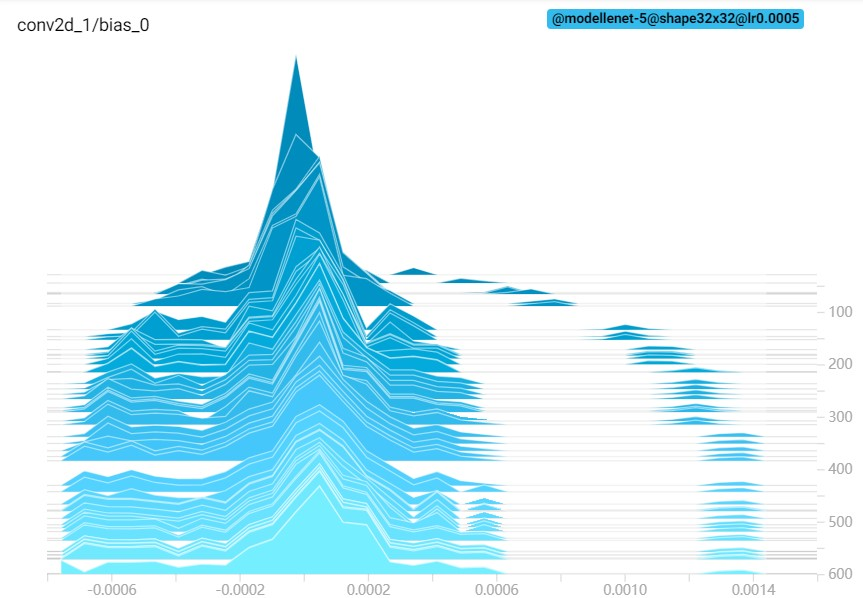
\includegraphics[width=.45\textwidth]{resource/analysis/histograms_lenet_conv2d_1_bias_0.jpg}
      }
      \subfigure[本文模型]{
        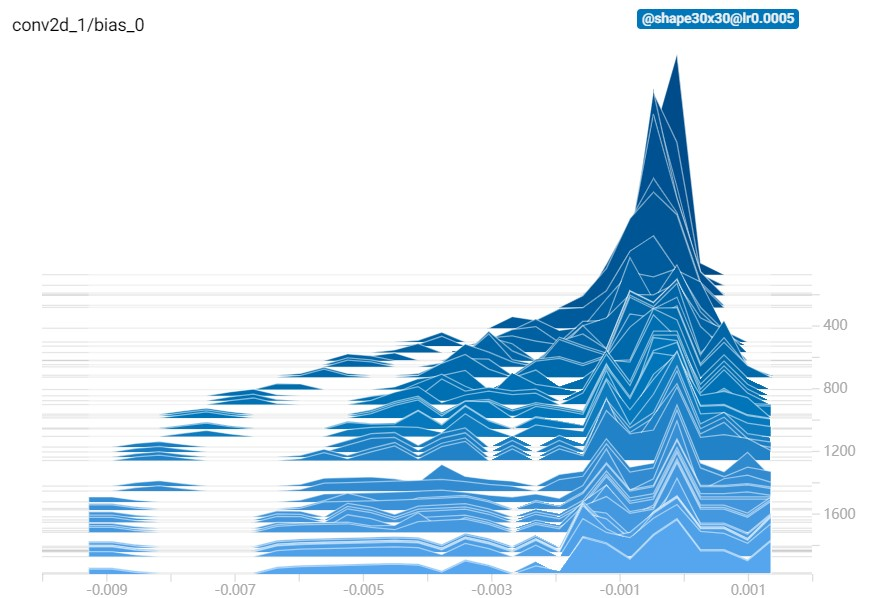
\includegraphics[width=.45\textwidth]{resource/analysis/histograms_newbnet_conv2d_1_bias_0.jpg}
      }
      \caption{3D分布图}
      \label{Figure.Fourth.5}
    \end{figure}
  